\Introduction
%Что дает сегментация разных диапазонов
%Отличие скоплений в оптике и рентгене
\section{Скопления галактик}
В 2019 году произошел запуск космической обсерватории СРГ (Спектр-Рентген-Гамма) с телескопами 
eROSITA и ART-XC на борту. Основной задачей этих телескопов является создание обзора всего неба в 
рентгеновском диапазоне. Данные, полученные от этих телескопов будут использоваться для обнаружения 
астрономических объектов трёх категорий:

\begin{enumerate}
    \item Скопления галактик.
    \item Сверхмассивные чёрные дыры.
    \item Рентгеновские звёзды в галактике Млечный путь. 
\end{enumerate}

Наибольший интерес представляют скопления галактик. Скопления --- это гравитационно связанные 
системы, которые являются самыми большими динамически связанными структурами во Вселенной. 
Скопления галактик играют важную роль в задачах определения космологических параметров Вселенной. 
Например, зная расстояние до скопления и его красное смещение (параметр, по которому можно понять, 
как объект отдаляется от наблюдателя), можно уточнить постоянную Хаббла, входящую в закон Хаббла, 
который описывает скорость расширения Вселенной. Кроме того, соотношение компонент материи в 
скоплениях должно отражать средний состав Вселенной, что позволяет измерить вклад барионов в общую
плотность Вселенной.\\

Скопления галактик излучают энергию в разных диапазонах, и их можно наблюдать не только в 
рентгеновских данных. Однако рентгеновские данные являются лучшим источником информации о скоплениях,
так как в оптическом диапазоне наблюдается не только излучение далёких скоплений, но и свет 
ближайших звёзд из Млечного пути. Несмотря на это, исследование оптического диапазона тоже может 
принести результаты, так как можно исследовать области неба, где излучение Млечного пути 
сравнительно меньше. К тому же, можно использовать карты сегментации оптического диапазона как один 
из входных слоёв для нейросети, сегментирующей рентгеновские данные, и тем самым увеличить точность 
сегментации (но такой подход ещё требует проверки и тестирования).\\

\begin{figure}[h]
    \center{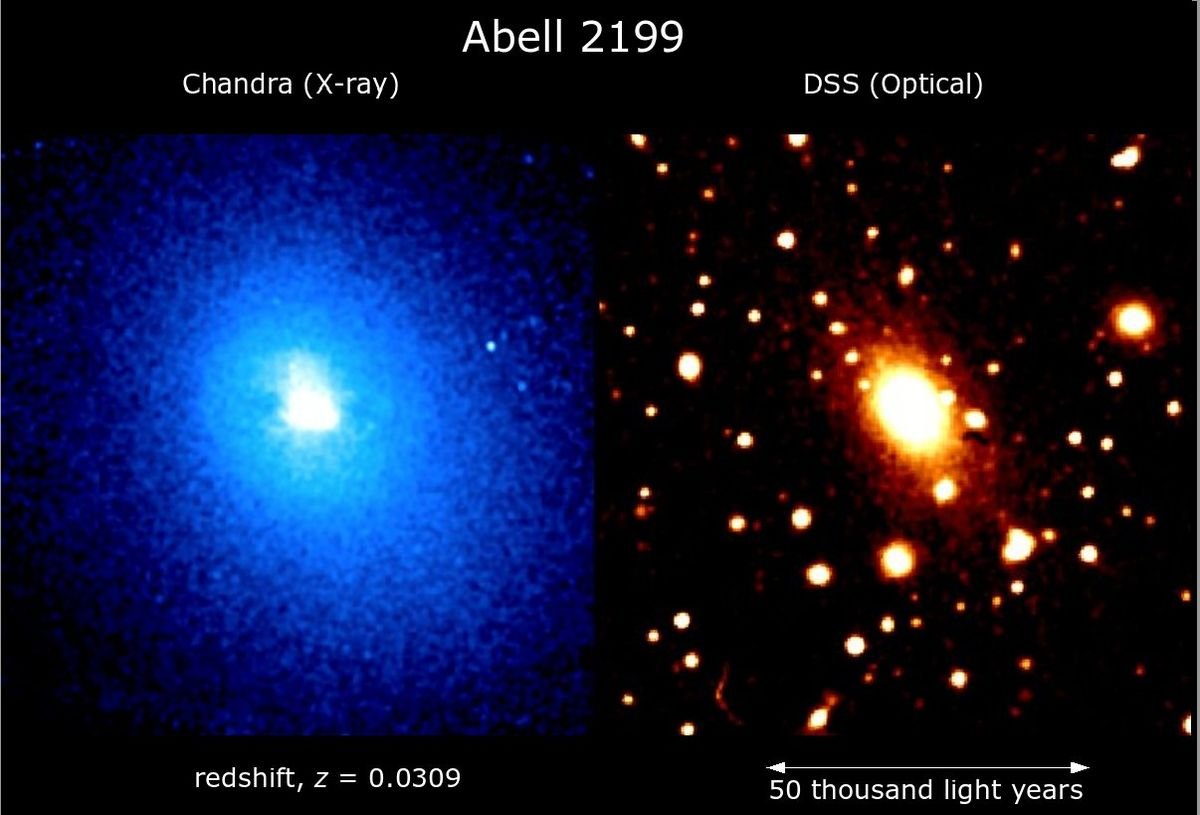
\includegraphics[width=0.7\linewidth]{comparison0}}
    \caption{Скопление <<Абель 2199>> в оптическом и рентгеновском диапазонах. \cite{Abell}}
\end{figure}

Полные обзоры неба, полученные телескопом eROSITA, появятся к июню 2020 года, поэтому на данный 
момент есть возможность подготовить модели для сегментации данных на примере других диапазонов.\\

В первую очередь будут использоваться данные оптического диапазона. Видимое излучение --- тот 
диапазон частот, что доступен глазу человека. На текущий момент существует большое количество 
оптических телескопов, и, как следствие, большое количество данных, извлеченных с их помощью. В 
данной работе будут использоваться данные телескопа Pan-STARRS1, который является частью системы 
телескопов Pan-STARRS (Panoramic Survey Telescope and Rapid Response System). Этот телескоп 
построен на вершине гавайского вулкана Халеакала. На 2007 год он обладал самой большой 
светочувствительной матрицей в мире. Кроме того, его данные находятся в общем доступе \cite{Panstarrs}.\\

\section{Нейросетевые методы}
В последние годы методы глубокого обучения стали играть важную роль в анализе данных. Нейросетевые 
модели показывают высокие результаты в области компьютерного зрения и в частности в задачах 
сегментации и детекции. Всё более часто они применяются и для решения задач астрофизики. 
Характеристики телескопа eROSITA позволят получить рентгеновские данные очень высокого качества (то 
есть с низким количеством шума), и методы глубокого обучения дают много преимуществ при анализе 
данных: 

\begin{enumerate}
    \item Стандартные алгоритмы сегментации усредняют информацию по нескольким каналам,
        в то время как с помощью нейросети можно охватить данные полностью и исследовать вопрос с 
        новой стороны. Таким образом, нейросеть будет получать <<сырые>> данные, что экономит время 
        и исключает необходимость контролировать процесс предобработки данных. 
        Кроме того, нейросеть, используя все данные, может получить информацию о 
        калибровке телескопа прямо из обзоров, что невозможно сделать при использовании классических 
        методов.
    \item Аналогичнные методы можно использовать для сегментации одновременно разнородных данных. 
        То есть для улучшения качества сегментации можно исследовать параллельно разные диапазоны 
        частот и находить взаимосвязь между разными спектрами.
    \item Каждый из классических методов имеет свои достоинства и недостатки, и для каждого 
        диапазона излучения существуют свои алгоритмы, в то время как 
        нейросеть может стать универсальным средством для сегментации.
\end{enumerate}

U-net \cite{Unet} является стандартной архитектурой для сегментации данных. Она идеально подходит 
для проверки идеи использования методов глубокого обучения для сегментации скоплений.
Её симметричная структура позволяет абстрагировать данные изображения, подаваемого на 
вход, в то время как skip-connection слои помогают увеличивать точность сегментации.

\begin{figure}[h]
    \center{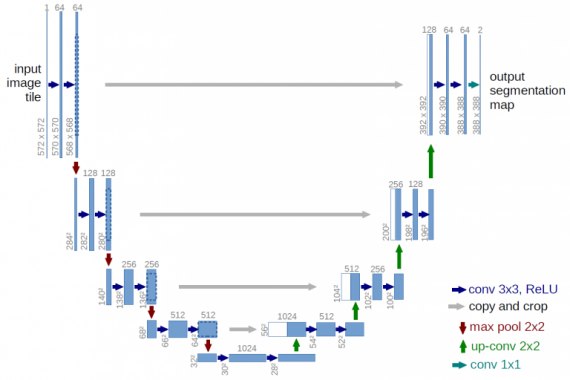
\includegraphics[width=0.7\linewidth]{unet0}}
    \caption{Структура модели U-net \cite{Unet}}
\end{figure}


